
\begin{center}
\thispagestyle{empty}

\vspace{.7cm}

% 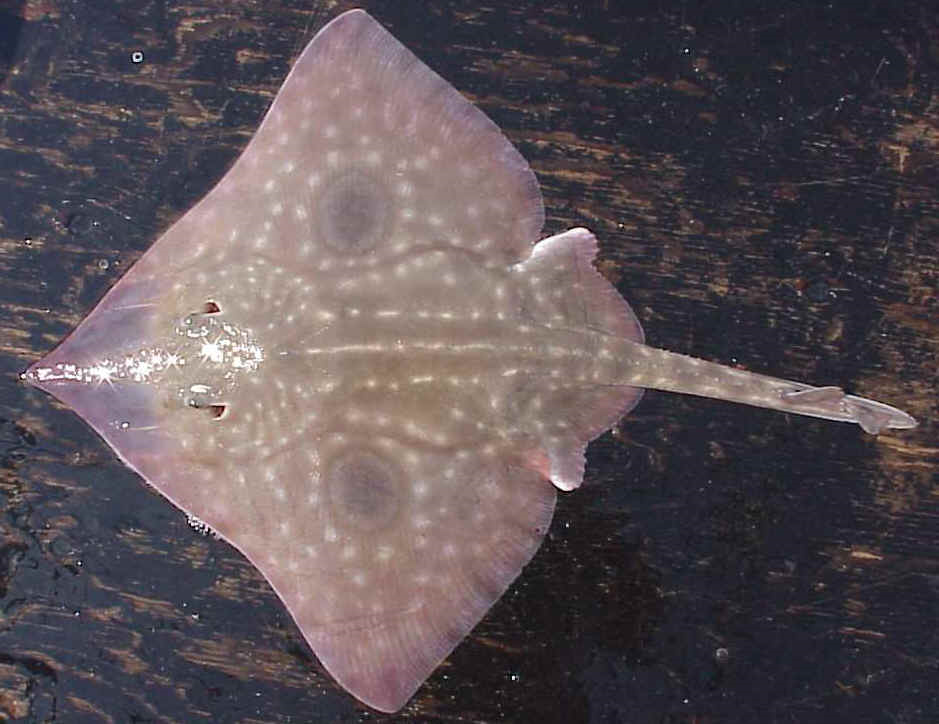
\includegraphics{cover_photo}~\\[1cm]
\pdftooltip{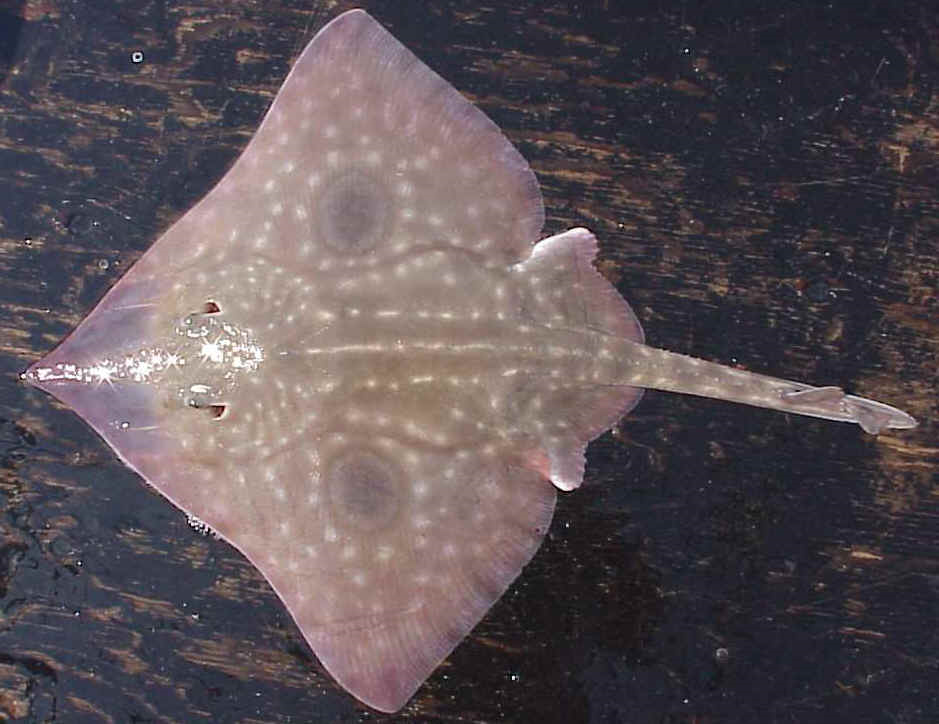
\includegraphics{cover_photo}}{This is a fish.}

\vspace{.5cm}

Ian G. Taylor\textsuperscript{1}\\
Vladlena Gertseva\textsuperscript{1}\\
Andi Stephens\textsuperscript{2}\\
Joseph Bizzarro\textsuperscript{3}\\

\vspace{.7cm}

\small

\textsuperscript{1}Northwest Fisheries Science Center, U.S. Department of Commerce, National Oceanic and Atmospheric Administration, National Marine Fisheries Service, 2725 Montlake Boulevard East, Seattle, Washington 98112\\

\vspace{.3cm}

\textsuperscript{2}Northwest Fisheries Science Center, U.S. Department of Commerce, National Oceanic and Atmospheric Administration, National Marine Fisheries Service, 2032 S.E. OSU Drive Newport, Oregon 97365

\vspace{.3cm}

\textsuperscript{3}Southwest Fisheries Science Center, U.S. Department of Commerce, National Oceanic and Atmospheric Administration, National Marine Fisheries Service, 110 Shaffer Road, Santa Cruz, California 95060\\



\vspace{.5cm}

\vfill
DRAFT SAFE\\
Disclaimer: This information is distributed solely for the purpose of pre-dissemination
peer review under applicable information quality guidelines. It has not been formally
disseminated by NOAA Fisheries. It does not represent and should not be construed to
represent any agency determination or policy. 

\vspace{.3cm}
%Bottom of the page
%{\large \today}


\newpage{\thispagestyle{empty}}

\vspace*{\fill}
\begin{flushleft}
This report may be cited as:

Taylor, I.G., Gertseva, V., Stephens, A. and Bizzarro, J. Status of Big Skate (\emph{Beringraja binoculata}) Off the U.S. West Coast, 2019. Pacific Fishery Management Council, Portland, OR. Available from http://www.pcouncil.org/groundfish/stock-assessments/
\end{flushleft}

\newpage{\thispagestyle{empty}}

\large{\textbf{Acronyms used in this Document}}

\vspace{.5cm}

\renewcommand{\arraystretch}{1.2}

\begin{table}[ht]
% \centering
\begin{tabular}{rll}
     & ABC & Allowable Biological Catch  \\ 
     & ACL  & Annual Catch Limit \\ 
     & ADFG & Alaska Department of Fish and Game \\ 
     & AFSC & Alaska Fisheries Science Center \\ 
     & A-SHOP & At-Sea Hake Observer Program  \\ 
     & CalCOM & California Cooperative Groundfish Survey  \\ 
     & CDFW & California Department of Fish and Wildlife  \\ 
     & CPFV & Commercial Passenger Fishing Vessel \\ 
     & CRFS & California Recreational Fisheries Survey \\ 
     & DFO & Canada’s Department of Fisheries and Oceans  \\ 
     & IFQ & Individual Fishing Quota \\ 
     & IPHC & International Pacific Halibut Commission \\ 
     & MRFSS & Marine Recreational Fisheries Statistics Survey  \\ 
     & NMFS & National Marine Fisheries Service  \\ 
     & NORPAC & the North Pacific Database Program \\ 
     & NWFSC & Northwest Fisheries Science Center  \\ 
     & ODFW & Oregon Department of Fish and Wildlife  \\ 
     & OFL & Overfishing Limit \\ 
     & ORBS & Oregon Recreational Boat Survey  \\ 
     & OY & Optimum Yield \\ 
     & PacFIN & Pacific Fisheries Information Network \\ 
     & PFMC & Pacific Fishery Management Council \\ 
     & PSMFC & Pacific States Marine Fisheries Commission  \\ 
     & RecFIN & Recreational Fisheries Information Network \\ 
     & SPR & Spawning Potential Ratio \\ 
     & SSC & Scientific and Statistical Committee \\ 
     & SWFSC & Southwest Fisheries Science Center  \\ 
     & WCGOP & West Coast Groundfish Observer Program  \\ 
     & WDFW & Washington Department of Fish and Wildlife  \\ 
\end{tabular}
\end{table}

\renewcommand{\arraystretch}{1}

\maketitle

\pagenumbering{roman}
\setcounter{page}{1}
\end{center}


